\section{Исследовательская часть}

В данном разделе будет проведено исследование разработанной программы. Будет верифицированна её работоспособность в различных конфигурациях системы. Также будут выявлены ограничения применимости приложения. Результаты всех экспериментов будут сопровождены выводами.  

\subsection{Постановка задачи}
С целью проверки работоспособности системы требуется исследовать зависимость стоимости начального оптимизированного плана от размерности системы.

Также необходимо произвести замеры среднего времени работы программы при разном количестве пунктов для определения ограничений её применимости.

С целью определения закономерностей работы системы будут проведены исследования зависимости общей стоимости маршрутов от следующих параметров:

\begin{enumerate}
	\item вместительность грузовика;	
\end{enumerate}

\subsection{Генерация системы}
Для проведения экспериментов необходимо иметь описания большого количества транспортных систем. Собрать большое количество реальных данных крайне затруднительно. Поэтому более предпочтительной является генерация случайной транспортной системы.

При генерации сети в первую очередь с помощью библиотеки networkx создаётся случайный граф. Полученные позиции вершин и их наличие рёбер между ними используется для создания дорог в транспортной системе. После этого узлам графа случайным образом сопоставляется роль пункта, набор продуктов в заказе или запасах.

Пример использования сгенерированной системы приведён на рисунке \ref{demo:routes2}.

\subsection{Проведение экспериментов}

\subsubsection{Исследование работы алгоритма}
Метод потенциалов является многоитерационным, поэтому имеется возможность проанализировать за счёт чего достигается более оптимальный план. В данном эксперименте будет исследованна зависимость стоимости маршрутов, их количества, средней длине и средней загруженности от текущей итерации оптимизации. Результат проведённого на случайной транспортной системе эксперимента изображён в виде графика на рисунке \ref{exp:iter}.

\begin{figure}[h!]
	\begin{center}
		{\includegraphics[scale=0.525, angle=0, page=1]{research/one_case_200.pdf}}
		\caption{Сравнение стоимостей плана до и после оптимизации}
		\label{exp:iter}
	\end{center}
\end{figure}

Из данного графика можно сделать вывод о том, что главным образом снижение стоимости достигается за счёт снижения общего числа маршрутов посредством продлении и распределения груза на другие маршруты.

\subsubsection{Сравнение плана до и после оптимизации}
Главным показателем корректности реализованного метода является наличие оптимизации. Оно выражается в том, что конечный план должен обладать меньшей суммарной стоимостью для всех маршрутов по сравнению с начальным, опорным планом. 

Чтобы установить выполнение данного условия в общем случае, в данном эксперименте были использованы случайно созданные транспортные сети размером от 20 до 85 пунктов. Измерения для каждой размерности проводятся многократно для усреднения полученных значений. Результат проведённого эксперимента изображён на графике, на рисунке \ref{exp:cmp}.

\begin{figure}[h!]
	\begin{center}
		{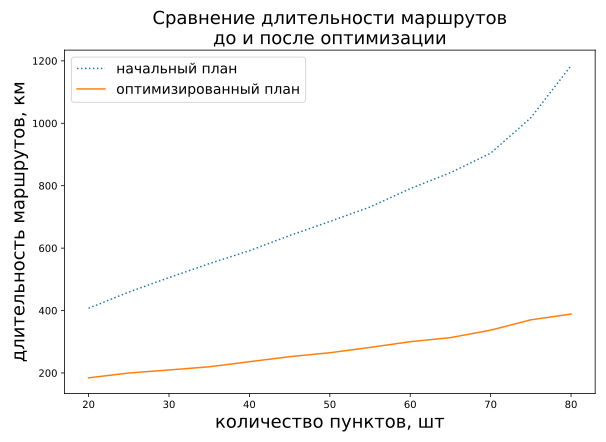
\includegraphics[scale=0.5, angle=0, page=1]{research/cmp.pdf}}
		\caption{Сравнение стоимостей плана до и после оптимизации}
		\label{exp:cmp}
	\end{center}
\end{figure}

Данный график показывает, что при любом рассмотренном размере оптимизация опорного плана сокращает стоимость грузоперевозок как минимум вдвое, из чего можно заключить, что метод является работоспособным.

\subsubsection{Определение ограничений программы}
Основным ограничением в работе программы может являться рост процессорного времени при увеличении размерности системы. Для определения существенности данного ограничения следует провести эксперимент по установлению зависимости времени обработки входных данных от их размера.

Для этого будут использованы случайно сгенерированные транспортные системы размером от 20 до 140 узлов. Результат проведённого эксперимента сведён в график, изображённый на рисунке \ref{exp:timing}.

\begin{figure}[h!]
	\begin{center}
		{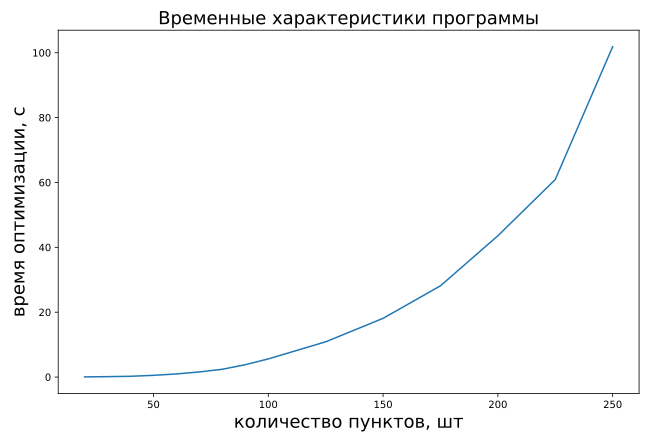
\includegraphics[scale=0.5, angle=0, page=1]{research/timing.pdf}}
		\caption{Зависимость времени работы от размерности}
		\label{exp:timing}
	\end{center}
\end{figure}

Из графика можно сделать вывод о том, что характер роста функции является нелинейным. При размере сети менее 50 пунктов время оптимизации составляет менее одной секунды. Большее количество узлов приводит к значительному росту времени обработки. Можно сделать вывод о том, что программа завершает оптимизацию за приемлемое время при размере сети до 150 узлов. 

Ввиду того, что сети подобного размера едва ли могут встретиться на практике, а также ввиду допустимости сравнительно длительного времени работы программы, полученные характеристики можно считать приемлимыми для выполнения поставленной задачи.

\subsubsection{Выявление закономерностей работы системы}
Разработанная программа позволяет моделировать поведение транспортной системы при изменении некоторых параметров. Рассмотрим некоторые из них.

В данном эксперименте изучается влияние вместительности грузовика на стоимость грузоперевозок. Размер системы принят равным 50 пунктам. Средний заказ имеет объём в 1м$^3$. Результат эксперимента приведён на рисунке \ref{exp:truck_vol}.

\begin{figure}[h!]
	\begin{center}
		{\includegraphics[scale=0.5, angle=0, page=1]{research/truck_vol.pdf}}
		\caption{Зависимость стоимости маршрутов от вместительности грузовиков}
		\label{exp:truck_vol}
	\end{center}
\end{figure}

Из данного графика видно, что использование грузовиков меньше объёма одного заказа невыгодно. Наиболее оптимальным в данной системе является использование грузовиков, способных вместить более четырёх заказов.


\subsection*{Вывод}
В данном разделе были описаны цели и планы проводимых экспериментов. В их рамках были проанализированны изменения различных параметров системы при работе алгоритма оптимизации, экспериментально обоснованна работоспособность метода. Были выявленны ограничения для использования разработанной программы, а также некоторые закономерности работы транспортной системы, на основе которых были предложены рекомендации по организации грузоперевозок. 

\pagebreak